% !TEX TS-program = pdflatex
% !TEX encoding = UTF-8 Unicode

% This is a simple template for a LaTeX document using the "article" class.
% See "book", "report", "letter" for other types of document.

\documentclass[11pt]{article} % use larger type; default would be 10pt

\usepackage[utf8]{inputenc} % set input encoding (not needed with XeLaTeX)

%%% Examples of Article customizations
% These packages are optional, depending whether you want the features they provide.
% See the LaTeX Companion or other references for full information.

%%% PAGE DIMENSIONS
\usepackage{geometry} % to change the page dimensions
\geometry{a4paper} % or letterpaper (US) or a5paper or....
% \geometry{margin=2in} % for example, change the margins to 2 inches all round
% \geometry{landscape} % set up the page for landscape
%   read geometry.pdf for detailed page layout information
\sloppy
\setlength{\parindent}{0pt}

\usepackage{graphicx} % support the \includegraphics command and options
\usepackage{bm}
\usepackage{amsmath}
\usepackage{amsfonts}
\usepackage{parskip}
\usepackage{graphicx}

% \usepackage[parfill]{parskip} % Activate to begin paragraphs with an empty line rather than an indent

%%% PACKAGES
\usepackage{booktabs} % for much better looking tables
\usepackage{array} % for better arrays (eg matrices) in maths
\usepackage{paralist} % very flexible & customisable lists (eg. enumerate/itemize, etc.)
\usepackage{verbatim} % adds environment for commenting out blocks of text & for better verbatim
\usepackage{subfig} % make it possible to include more than one captioned figure/table in a single float
% These packages are all incorporated in the memoir class to one degree or another...

%%% HEADERS & FOOTERS
\usepackage{fancyhdr} % This should be set AFTER setting up the page geometry
\pagestyle{fancy} % options: empty , plain , fancy
\renewcommand{\headrulewidth}{0pt} % customise the layout...
\lhead{}\chead{}\rhead{}
\lfoot{}\cfoot{\thepage}\rfoot{}

%%% SECTION TITLE APPEARANCE
\usepackage{sectsty}
\allsectionsfont{\sffamily\mdseries\upshape} % (See the fntguide.pdf for font help)
% (This matches ConTeXt defaults)

%%% ToC (table of contents) APPEARANCE
\usepackage[nottoc,notlof,notlot]{tocbibind} % Put the bibliography in the ToC
\usepackage[titles,subfigure]{tocloft} % Alter the style of the Table of Contents
\renewcommand{\cftsecfont}{\rmfamily\mdseries\upshape}
\renewcommand{\cftsecpagefont}{\rmfamily\mdseries\upshape} % No bold!

%%% END Article customizations

%%% The "real" document content comes below...

\title{Computational Stochastic Processes - Project 2}
\author{Tom McGrath}
%\date{} % Activate to display a given date or no date (if empty),
         % otherwise the current date is printed 

\begin{document}
\maketitle

\section{Question 1}
\subsection{Q1 (a)}
I solved the SDE:
\[
	d\mathbf{X}_{t} = \mathbf{v}(t, \mathbf{X}_{t})dt + \sqrt{2\kappa}dW_{t}, \quad \mathbf{X}_{0} = \mathbf{x}
\]
where $\mathbf{v}(t,\mathbf{x})$ is given by:
\[
	\mathbf{v}(t,\mathbf{x}) = (0,\,\sin(x)\sin(\omega t))
\]
using the Euler-Marayama scheme with a stepsize of $\delta t = 0.01$ and $T = 1000$ we can simulate paths of the solution to the SDE, and so calculate $D(t)$:
\[
	D(t) = \frac{Var(Y_{t})}{2t}
\]
calculating the mean of $D(t)$ over [N] runs gives:
\begin{figure}
	\centering
		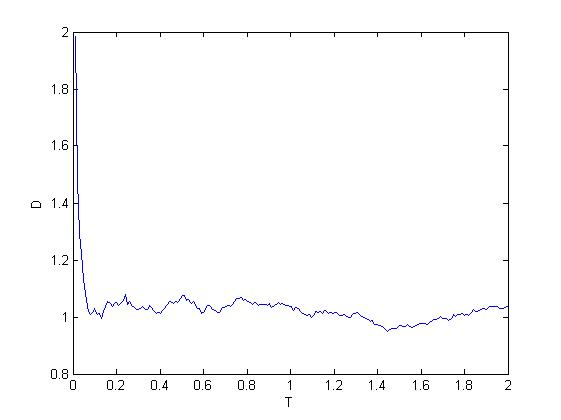
\includegraphics[scale = 0.5]{q1.jpg}
		\caption{The diffusion coefficient D tends to a constant value at T becomes large}
\end{figure}
Varying $\kappa$ and $\omega$ between $10^{-2}$ and $10^{2}$ we obtain the following results  for $D(t)$:
\begin{figure}
	\centering
		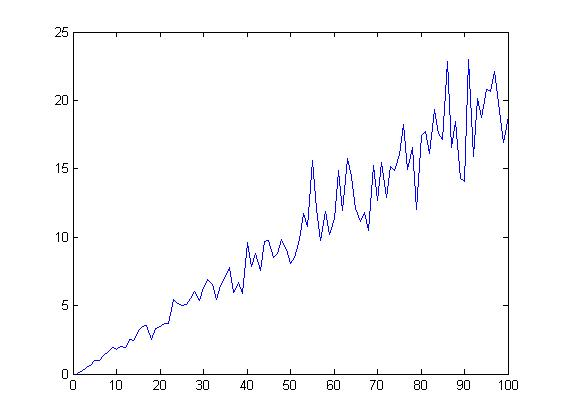
\includegraphics[scale = 0.5]{q1a_kappa.jpg}
		\caption{Dependence of D on $\kappa$}
\end{figure}
\begin{figure}
	\centering
		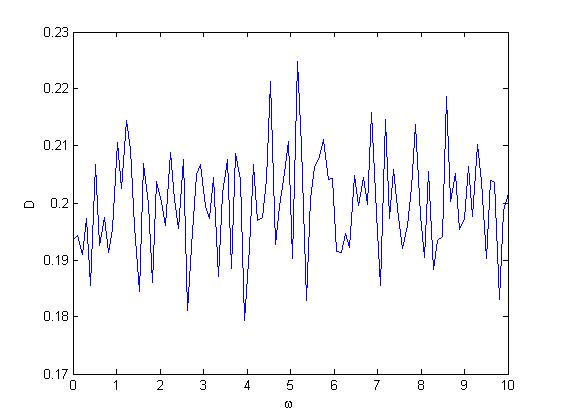
\includegraphics[scale = 0.5]{q1a_omega}
		\caption{Dependence of D on $\omega$}
\end{figure}
\subsection{Q1(b)}
Now we have  $\mathbf{v}(t,\mathbf{x})$ defined as:
\[
	\mathbf{v}(t,\mathbf{x}) = (0,\, \sin(x)\eta_{t})
\]
with $\eta_{t}$ given by the SDE:
\[
	d\eta_{t} = -\alpha\eta_{t}dt + \sqrt{2\alpha}dW_{t}, \quad \eta_{0} \sim \mathcal{N}(0,1)
\]
Now as we vary $\kappa$ and $\alpha$ in the range $[10^{-2}, 10^{2}]$ the diffusion coefficient at time $T = 1000$ varies as shown in the figures below:
\begin{figure}
	\centering
		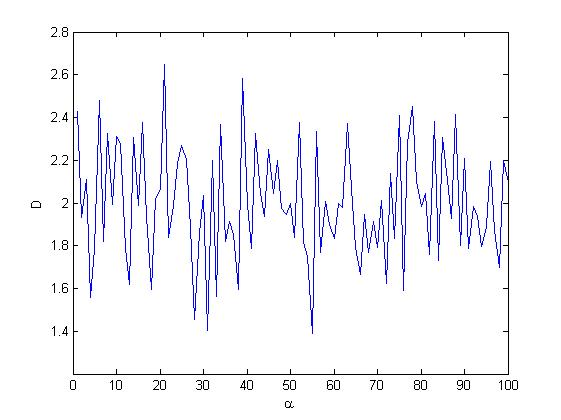
\includegraphics[scale = 0.5]{q1b_alpha}
		\caption{Dependence of D on $\alpha$}
\end{figure}

\begin{figure}
	\centering
		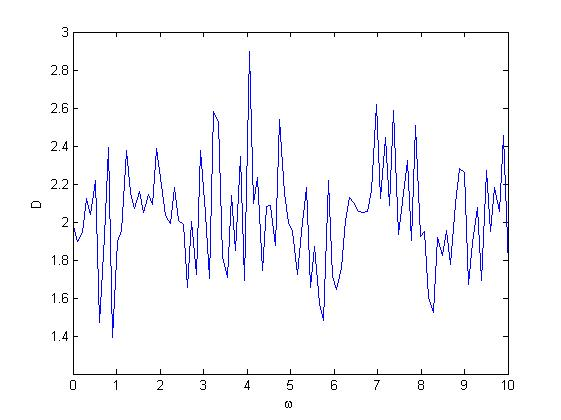
\includegraphics[scale = 0.5]{q1b_kappa}
		\caption{Dependence of D on $\kappa$}
\end{figure}
\section{Question 2}
The system of SDEs:
\begin{align}
	\frac{dx_{t}}{dt} &= \frac{x_{t}y_{t}}{\epsilon} - y_{t}^{2}x_{t}^{3}\\
	dy_{t} &= -\frac{1}{\epsilon^{2}}y_{t}dt + \frac{\sqrt{2}}{\epsilon}dW_{t}, \quad y_{0}\sim\mathcal{N}(0,1)
\end{align}
converges to the SDE:
\[
	dX_{t} = (X_{t} - X_{t}^{3})dt + \sqrt(2)X_{t}dW_{t},\quad X_{0} = 1
\] the 
which is an SDE for a particle moving in a bistable potential well with multiplicative noise. In the case of additive noise, the particle stays well-confined to each well, and occasionally switches depending on the strength of the noise. I would expect the multiplicative noise case to be less stable as deviations are reinforced by the multiplicative noise.
\subsection{Q2 (a)}
We can use implicit or explicit schemes easily for $y_{t}$ as it is linear, however simulating the process to which the system converges  ($X_{t}$) implicitly is less simple, as the nonlinear relationship means we cannot rearrange to find $X_{n+1}$ as a function of $X_{n}$. We could use a Newton-Raphson root finder to solve this equation (as I've done in the Mastery question) but when I wrote the code I hadn't realised this so used the explicit form.


I have written explicit and semi-implicit EM solvers as well as an explicit Milstein scheme for $y_{t}$ and an explicit Milstein scheme for $X_{t}$. The equation $x_{t}$ is deterministic given $y_{t}$ so I simply used an Euler scheme to solve this. I tried also using an Euler scheme to simulate $X_{t}$ however the stability properties for the nonlinear equation are significantly less good so chose a Milstein scheme instead.

\subsection{Q2 (b)}
Using the explicit Milstein scheme I simulated both processes (using the same noise for each pair of paths) to investigate the error:
\[
	err(\epsilon) = E|x_{T} - X_{T}|^{2}
\]
and found the following dependence:
\begin{figure}
	\centering
		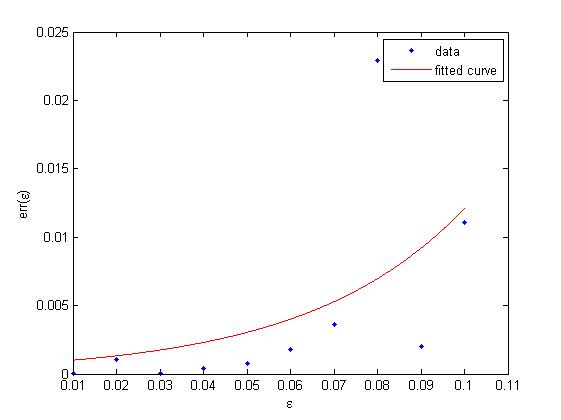
\includegraphics[scale = 0.5]{q2_epsilon.jpg}
		\caption{Dependence of err($\epsilon$) on $\epsilon$}
\end{figure}
This is of the form:
\[
err(\epsilon) \simeq C\epsilon^{\gamma}
\]
where $\gamma \simeq -0.14$
\subsection{Q2 (c)}
Plotting $err(\epsilon)$ as $T$ increases gives the result:
\begin{figure}
	\centering
		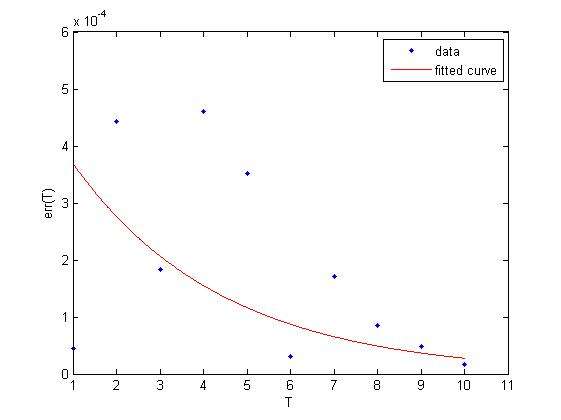
\includegraphics[scale = 0.5]{q2_T.jpg}
		\caption{Dependence of err on $T$}
\end{figure}
Error decays exponentially with time.
\section{Question 3}
\subsection{Q3 (a)}
For the scalar SDE:
\[
	dX_{t} = \lambda X_{t}dt+\sigma X_{t}dW_{t}
\]
we can find $E|X_{t}|^{2} = EX_{t}\bar{X_{t}}$ to determine the mean square stability condition. Using the generator of the process $\mathcal{L}$, determine $dX_{t}^{2}$:
\begin{align}
	dX_{t}^{2} &= \mathcal{L}X_{t}^{2} + \frac{\partial}{\partial x}X_{t}^{2}\sigma X_{t}dW_{t}\\
	&= \left( \lambda x \frac{\partial}{\partial x} + \frac{\sigma^{2}x^{2}}{2} \right)x^{2}(X_{t})dt + 2\sigma X_{t}^{2}dW_{t}
\end{align}
taking expectataion:
\begin{align}
	\mathbb{E}dX_{t}^{2} &= \mathbb{E}(2\lambda X_{t}^{2} + \sigma^{2}X_{t}^{2})dt + 2\sigma X_{t}^{2}dW_{t}\\
	& = (2\lambda + \sigma^{2})\mathbb{E}X_{t}^{2}dt
\end{align}
so
\[
	\frac{d\mathbb{E}X_{t}^{2}}{dt} = (2\lambda + \sigma^{2})\mathbb{E}X_{t}^{2}
\]
which implies a solution:
\[
	\mathbb{E}X_{t}^{2} = \mathbb{E}X_{0}^{2}e^{(2\lambda + \sigma^{2})t}
\]
if we want mean-squared stability, we need $\mathbb{E}X_{t}^{2}\to 0$ as $t\to\infty$, so $2\Re(\lambda) + |\sigma|^{2} < 0$
\subsection{Q3 (b)}
Writing out the $\theta$ Milstein scheme applied to the scalar SDE:
\[
X_{n+1} = X_{n} + \theta\lambda\Delta t X_{n+1} + (1-\theta)\lambda\Delta t X_{n} + \sigma X_{n}\Delta t^{\frac{1}{2}}\xi_{n} + \frac{1}{2}\sigma^{2}X_{n}(\sigma^{2}\Delta t(\xi - 1))
\]
rearranging gives the recurrence formula for the $\theta$ Milstein scheme:
\[
	X_{n+1} = G(\Delta t,\lambda,\sigma,\theta)X_{n}
\]
where $G(\Delta t,\lambda,\sigma,\theta)$ is given by:
\[
	\frac{1 + (1-\theta)\lambda\Delta t + \sigma\Delta t^{\frac{1}{2}}\xi_{n} + \frac{1}{2}\sigma^{2}(\Delta t(\xi^{2} -1)}{1-\theta\lambda\Delta t}
\]
which agrees with the answer given by Higham in 'A-Stability and Stochastic Mean-Square Stability' (SIAM J Numer Anal, 1996), whose derivation I will follow for the region of mean-squared stability. Defining:
\begin{align}
	p &= \frac{1 + (1-\theta)\lambda\Delta t - \frac{1}{2}\sigma^{2}\Delta t}{1-\theta\lambda\Delta t}\\
	q &= \frac{\Delta t^{\frac{1}{2}}\sigma}{1-\theta\lambda\Delta t}\\
	r &= \frac{\frac{1}{2}\Delta t \sigma^{2}}{1-\theta\lambda\Delta t}
\end{align}
and taking the expectation of the modulus squared ($\mathbb{E}\xi = 0$, $\mathbb{E}\xi^{2} = 1$, $\mathbb{E}\xi^{3} = 0$, $\mathbb{E}\xi^{4} = 3$) gives:
\[
	\mathbb{E}|X_{n+1}|^{2} = (|p + q|^{2} + |q|^{2} + 2|r|^{2})\mathbb{E}|X_{n}|^{2}
\]
which is true if:
\[
	|p + q|^{2} + |q|^{2} + 2|r|^{2} < 1
\]
so substituting back values for $p$, $q$ \& $r$:
\[
	\Re(\lambda) + \frac{1}{2}|\sigma|^{2} + \frac{1}{2}\Delta t((1-2\theta) |\lambda|^{2} + \frac{1}{2}|\sigma|^{4}) < 0
\]
i.e. we have mean squared stability when
\[
	\Re(\lambda) + \frac{1}{2}|\sigma|^{2} + \frac{1}{4}\Delta t|\sigma|^{4} < \frac{1}{2}\Delta t(2\theta - 1)|\lambda|^{2}
\]
giving a condition on $\theta$ of:
\[
	\theta > \frac{\Re(\lambda) + \frac{1}{2}|\sigma|^{2} + \frac{1}{4}\Delta t|\sigma|^{4} + \frac{1}{2}\Delta t \lambda^{2}}{\Delta t}
\]
\subsection{Q3 (c)}
For the case $\lambda = -100$, $\sigma = 10$, and $\Delta t = 0.01$ with 1000 runs the mean given by the semi-implicit Milstein scheme with $\theta = 0.5$ is plotted below:
\begin{figure}
	\centering
		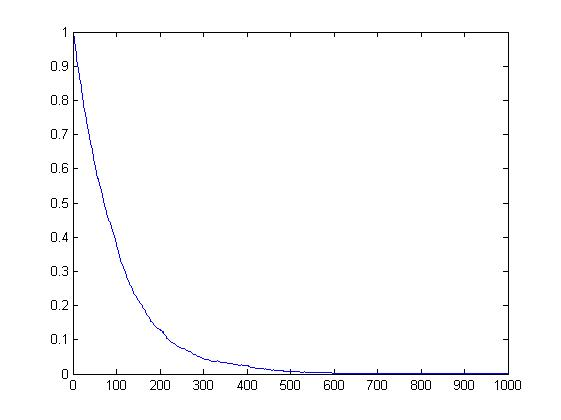
\includegraphics[scale = 0.5]{q3_meanX}
		\caption{Mean of semi-implicit Milstein scheme}
\end{figure}
This is inside the region of mean squared stability, and has stable behaviour. I haven't had time to test a variety of values of $\lambda$, $\theta$, $\sigma$ and $\Delta t$ but it would be sensible to obtain values around the boundary between expected mean-square stability and not. With $\lambda = -100 + 100i$, the path of the mean in the complex plane is:
\begin{figure}
	\centering
		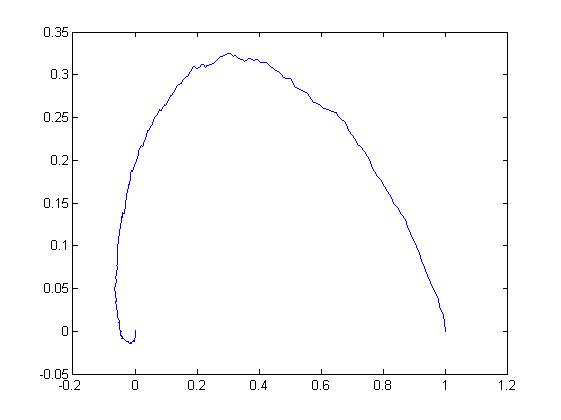
\includegraphics[scale = 0.5]{q3_meanCom}
		\caption{Mean value of semi-implicit Milstein scheme with complex $\lambda$}
\end{figure}
\section{Mastery Question}
\subsection{MQ (a)}
Consider the SDE:
\[
	dX_{t} = -\lambda X_{t}(1-X_{t})\,dt - \mu X_{t}(1-X_{t})\,dW_{t}
\]
linearising by $X_{t} \to 1 + x_{t}$ and retaining only terms linear in $x_{t}$:
\[
	-\lambda X_{t}(1-X_{t}) \to -\lambda(1+x_{t})(1 - 1 + x_{t}) \simeq -\lambda x_{t}
\]
(and likewise for the noise term) gives the SDE of geometric BM:
\[
	dX_{t} = -\lambda X_{t}dt - \mu X_{t}dW_{t}
\]
\subsection{MQ (b)}
Solving (5) with the explicit Euler scheme for $\lambda = -1$, $X_{0} = 1.1$ and $\mu = 0.5, 0.6, 0.7, 0.8, 0.9$ gives results for $\mathbb{E}(X_{t} - 1)^{2}$. As $\mu$ increases, the mean squared error also increases.
\begin{figure}
	\centering
		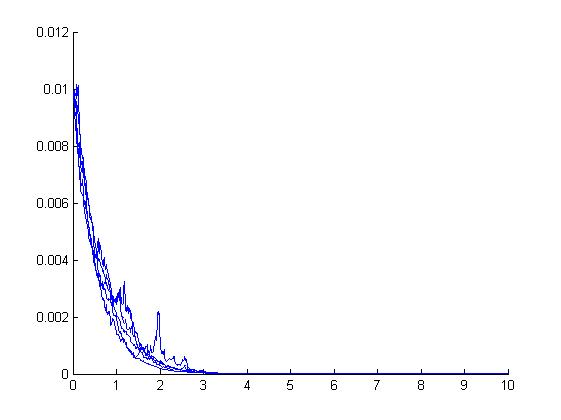
\includegraphics[scale = 0.5]{MQ_exEM.jpg}
		\caption{MSE for explicit EM scheme}
\end{figure}
With the explicit Milstein scheme the MSE falls away rapidly, so I have zoomed in on the region $[0,0.2]$:
\begin{figure}
	\centering
		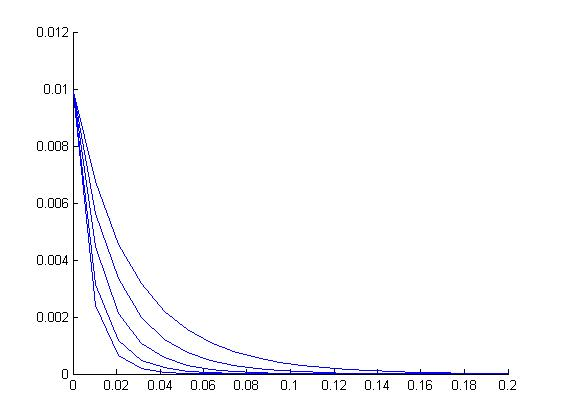
\includegraphics[scale = 0.5]{MQ_stocM}
		\caption{MSE for explicit Milstein scheme}
\end{figure}

\subsection{MQ (c)}
Using the theta scheme initially presents a problem as when we rearrange the stochatic theta scheme recurrence relation we get a nonlinear equation, so we cannot simply enter the values of the constants and calculate $X_{n+1}$. Instead, at each step we need to find the root of a nonlinear equation. Defining an anonymous function inline and using MATLAB's root-finding routine allows us to do this quickly \& accurately. The mean square stability properties of the stochastic $\theta$ scheme are considerably better for high $\mu$ than those of explicit schemes. We obtain the following results for mean squared error:
\begin{figure}
	\centering
		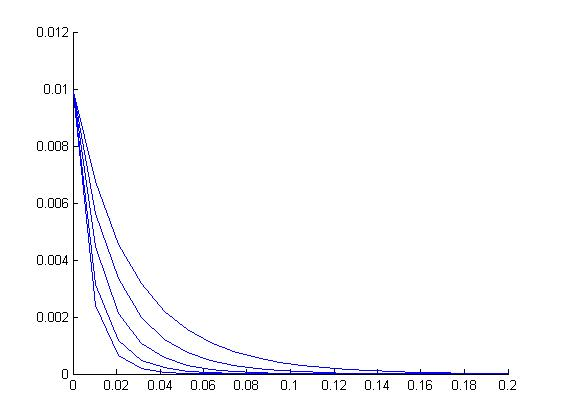
\includegraphics[width = 0.9\textwidth]{MQ_stocM.jpg}
		\caption{MSE for semi-implicit Milstein scheme with $\theta = 0.5$}
\end{figure}

\section{Code}
I have also written some 'wrapper' code to deal with the business of processing the outputs into answers for the questions but it's not particularly interesting so there seemed no point in bulking this file out more by putting them in.
\subsection{Q1}
    \begin{verbatim}
function [ D_T ] = q1afn( kappa, omega )

numRuns = 1000;
Tmax = 100; dt = 0.01;
T = linspace(0,Tmax,Tmax/dt);
dWX = sqrt(dt)*randn(numRuns,length(T)); % vectorise for speed
dWY = sqrt(dt)*randn(numRuns,length(T));
X = zeros(numRuns,length(T)); % initialise for speed
Y = zeros(numRuns, length(T));
D = zeros(1,length(T));
x0 = 1.0;
y0 = 1.0;

for i = 1:numRuns
    X_j = x0;
    Y_j = y0;
    for j = 1:length(T)
       incY =  sqrt(2.0*kappa)*dWY(i,j);
       Y_j = Y_j + sin(X_j)*sin(omega*(j*dt)) + incY;
       Y(i,j) = Y_j;
       incX = sqrt(2.0*kappa)*dWX(i,j);
       X_j = X_j + incX;
       X(i,j) = X_j;
    end
end

D = var(X)./(2*T);
D_T = D(length(T));

end
\end{verbatim}

    \begin{verbatim}
function [ D_T ] = q1bfn( kappa, alpha )

numRuns = 100;
Tmax = 1000; dt = 0.01;
T = linspace(0,Tmax,Tmax/dt);
dWX = sqrt(dt)*randn(numRuns,length(T)); % vectorise for speed
dWY = sqrt(dt)*randn(numRuns,length(T));
dWEta = sqrt(dt)*randn(numRuns,length(T));
X = zeros(numRuns,length(T)); % initialise for speed
Y = zeros(numRuns, length(T));
eta = zeros(numRuns, length(T));
x0 = 1.0;
y0 = 1.0;

% all schemes currently explicit method, could adapt eta and y to implicit
% EM or Milstein easily as they are linear
for i = 1:numRuns
    X_j = x0;
    X(i,1) = X_j;
    Y_j = y0;
    Y(i,1) = Y_j;
    eta_j = randn();
    eta(i,1) = eta_j;
    for j = 2:length(T)
       incY =  sqrt(2.0*kappa)*dWY(i,j);
       Y_j = Y_j + sin(X_j)*eta_j*dt + incY;
       Y(i,j) = Y_j;
       incX = sqrt(2.0*kappa)*dWX(i,j);
       X_j = X_j + incX;
       X(i,j) = X_j;
       incEta = sqrt(2.0*alpha)*dWEta(i,j);
       eta_j = eta_j - alpha*eta_j*dt + incEta;
       eta(i,j) = eta_j;
    end
end

D = var(X)./T;
D_T = D(length(T));

end
\end{verbatim}

\section{Q2}
    \begin{verbatim}
function [ errT ] = q2fn( Tmax, dt, epsilon )
numRuns = 500;
theta = 1.0;
T = linspace(0,Tmax,Tmax/dt);
dW = randn(numRuns,length(T));
X = zeros(numRuns,length(T));
Y = zeros(numRuns,length(T));
Z = zeros(numRuns,length(T));

% % use Milstein scheme on Y - equivalent to EM as sigma' = 0
% for i = 1:numRuns
%     Y_j = randn();
%     Y(i,1) = Y_j;
%     for j = 2:length(T)
%         Y_j = Y_j - Y_j*(dt/epsilon)/epsilon + (sqrt(2)/epsilon)*sqrt(dt)*dW(i,j);
%         %Y_j = Y_j - Y_j*(dt/(epsilon^2)) + (sqrt(2)/epsilon)*sqrt(dt)*dW(i,j);
%         Y(i,j) = Y_j;
%     end
% end

% use implicit EM scheme on Y
for i = 1:numRuns
    Y_j = randn();
    Y(i,1) = Y_j;
    for j = 2:length(T)
        Y_j = (1/(1+((theta*dt)/(epsilon^2))))*(Y_j - (1-theta)*Y_j*dt/(epsilon^2) + (sqrt(2)/epsilon)*sqrt(dt)*dW(i,j));
        Y(i,j) = Y_j;
    end
end

% % use stochastic theta with EM scheme to obtain y series first
% for i = 1:numRuns
%     Y_j = randn();
%     Y(i,1) = Y_j;
%     for j = 2:length(T)
%         Y_j = (epsilon^2/(epsilon^2+theta))*Y_j + ((theta - 1)/(epsilon^2 + theta))*Y_j*dt + (sqrt(2)/(epsilon + (theta/epsilon)))*dW(i,j);
%         Y(i,j) = Y_j;
%     end
% end

% now solve the equation in x using the y series
for i = 1:numRuns
    X_j = 1.0;
    X(i,1) = X_j;
    for j = 2:length(T)
        X_j = X_j + ((X_j*Y(i,j))/epsilon)*dt - ((X_j^3)*(Y(i,j)^2))*dt;
        X(i,j) = X_j;
    end
end

% using explicit Milstein for eq(2c)
for i = 1:numRuns
    Z_j = 1.0;
    Z(i,1) = 1.0;
    for j = 2:length(T)
        Z_j = Z_j + (Z_j - Z_j^3)*dt + sqrt(2)*Z_j*sqrt(dt)*dW(i,j) + Z_j*dt*(dW(i,j)*dW(i,j) - 1);
        Z(i,j) = Z_j;
    end
end

err = (Z - X);
err = err.^2;
errT = err(length(T));
%mErr = mean(err);
%errT = mErr(length(T));

hold on
for i = 1:numRuns
   %plot(Z(i,:), 'Color', 'green')
   %plot(Y(i,:), 'Color', 'blue')
   plot(X(i,:), 'Color', 'red')
   %plot(err(i,:))
end
% plot(mErr, 'Color', 'black')
% mErr(length(T))
% hold off
end

\section{Q3}

    
    \begin{verbatim}
numRuns = 100;
theta = 1.0;
lambda = -100;
mu = 10;
Tmax = 0.1;
dt = 0.01;
T = linspace(0,Tmax,Tmax/dt);
X = zeros(numRuns,length(T));
dW = randn(numRuns,length(T));

for i = 1:numRuns
    X_j = 1.0;
    X(i,1) = X_j;
    for j = 2:length(T)
        X_j = (X_j + (1-theta)*lambda*dt*X_j + mu*sqrt(dt)*X_j*dW(i,j) + 0.5*mu*mu*dt*X_j*(dW(i,j)*dW(i,j) - 1))/(1-theta*lambda*dt);
        X(i,j) = X_j;
    end
end

plot(mean(X))
\end{verbatim}


    
    \begin{verbatim}
function [ mErr ] = MQfn( Tmax,dt,mu )
numRuns = 100;
T = linspace(0,Tmax,Tmax/dt);
dW = randn(numRuns,length(T));
X = zeros(numRuns,length(T));
lambda = -1.0;
theta = 0.5;

% %EM scheme
% for i = 1:numRuns
%    X_j = 1.1;
%    X(i,1) = X_j;
%    for j = 2:length(T)
%       X_j = X_j - lambda*X_j*(1-X_j)*dt - mu*X_j*(1-X_j)*sqrt(dt)*dW(i,j);
%       X(i,j) = X_j;
%    end
% end

% %Milstein scheme
% for i = 1:numRuns
%    X_j = 1.1;
%    X(i,1) = X_j;
%    for j = 2:length(T)
%       X_j = X_j - lambda*X_j*(1-X_j)*dt - mu*X_j*(1-X_j)*sqrt(dt)*dW(i,j) - 0.5*(mu*mu*X_j*(1-X_j) - 2*mu*mu*X_j*X_j*(1-X_j));
%       X(i,j) = X_j;
%    end
% end

% semi-implicit Milstein scheme
for i = 1:numRuns
   X_j = 1.1;
   X(i,1) = X_j;
   for j = 2:length(T)
       % use anonymous function to define newton-raphson root quickly
       milstein = @(x) x*(1+theta*lambda*dt*(1-x)) - (X_j - lambda*X_j*(1-X_j)*dt - mu*X_j*(1-X_j)*sqrt(dt)*dW(i,j) - 0.5*(mu*mu*X_j*(1-X_j) - 2*mu*mu*X_j*X_j*(1-X_j)));
       x = fzero(milstein, X_j);
       X_j = x;
       X(i,j) = X_j;
   end
end

err = (X-1);
err = err.^2;
mErr = mean(err);

end
\end{verbatim}

\end{document}
